\documentclass[11pt,letterpaper]{article}
\usepackage[utf8]{inputenc}

%----- Configuración del estilo del documento------%
\usepackage{epsfig,graphicx}
\usepackage[left=2cm,right=2cm,top=1.8cm,bottom=2.3cm]{geometry}
\usepackage{fancyhdr}
\usepackage{lastpage}

\usepackage{xcolor}
\usepackage{soul}
\newcommand{\mathcolorbox}[2]{\colorbox{#1}{$\displaystyle #2$}}

%Color bibi
\definecolor{bibi}{RGB}{0,103,148}
% Otros colores

%------ Paquetes de dibujo --------%
\usepackage{tikz}
\usepackage{circuitikz}

%------ Paquetes para mantener las imágenes en su lugar --------%
\usepackage{float}

%------ Paquete para notacion de dirac -------%
\usepackage{braket}

%------ Paquetes para mantener las imágenes en su lugar --------%
\usepackage{float}

%------ Paquete para codigo 
\usepackage{minted}

\usepackage{cite}
\usepackage{multicol}
\setlength{\columnsep}{1.5cm}
\setlength{\columnseprule}{.5pt}

\pagestyle{fancy}
\fancyhf{}
\rfoot{\textit{Página \thepage \hspace{1pt} de \pageref{LastPage}}}

%------ Paquetes matemáticos básicos --------%
\usepackage{amsmath}
\usepackage{amssymb}
\usepackage{amsthm}

\begin{document}
%------ Encabezado -------- %
\begin{center}
    \begin{minipage}{3cm}
    	\begin{center}
    		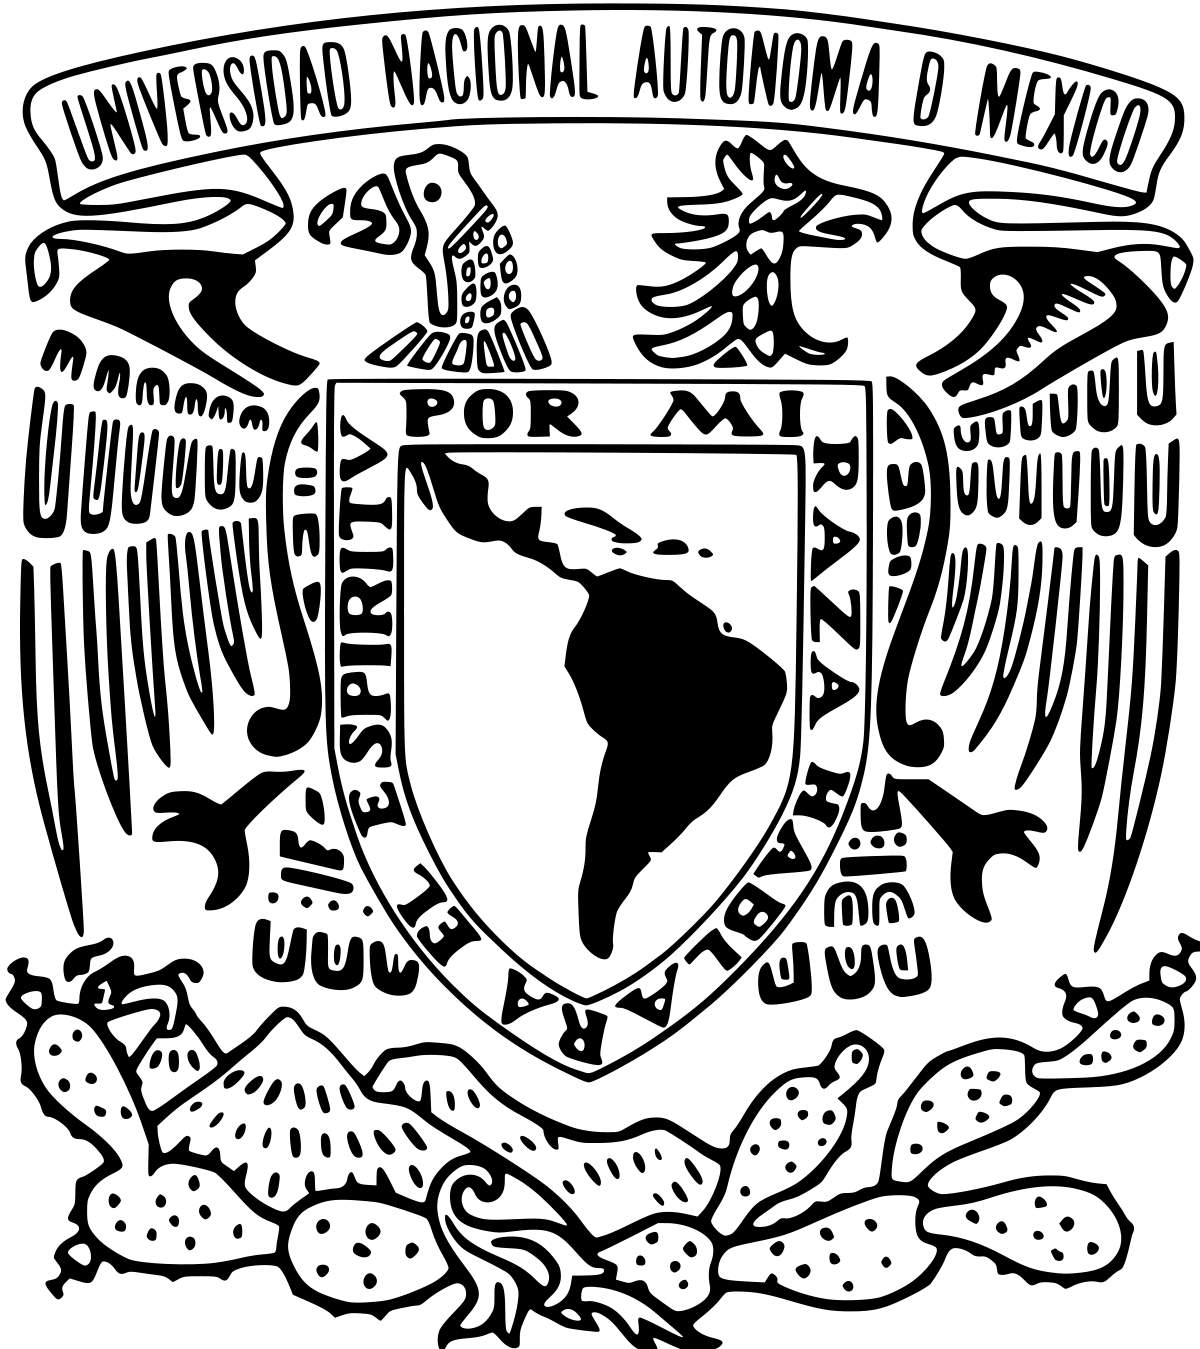
\includegraphics[height=3.3cm]{src/Img/Logo_UNAM.png}
    	\end{center}
    \end{minipage}\hfill
    \begin{minipage}{10cm}
    	\begin{center}
    	\textbf{\large Universidad Nacional Autónoma de México}\\[0.1cm]
        \textbf{Facultad de Ciencias}\\[0.1cm]
        \textbf{Criptografía y seguridad $|$ 7133}\\[0.1cm]
        Tarea corta 2 : $|$ Divisibilidad 9 \\[0.1cm]
        Sosa Romo Juan Mario $|$ 320051926 \\[0.1cm]
        16/09/24
    	\end{center}
    \end{minipage}\hfill
    \begin{minipage}{3cm}
    	\begin{center}
    		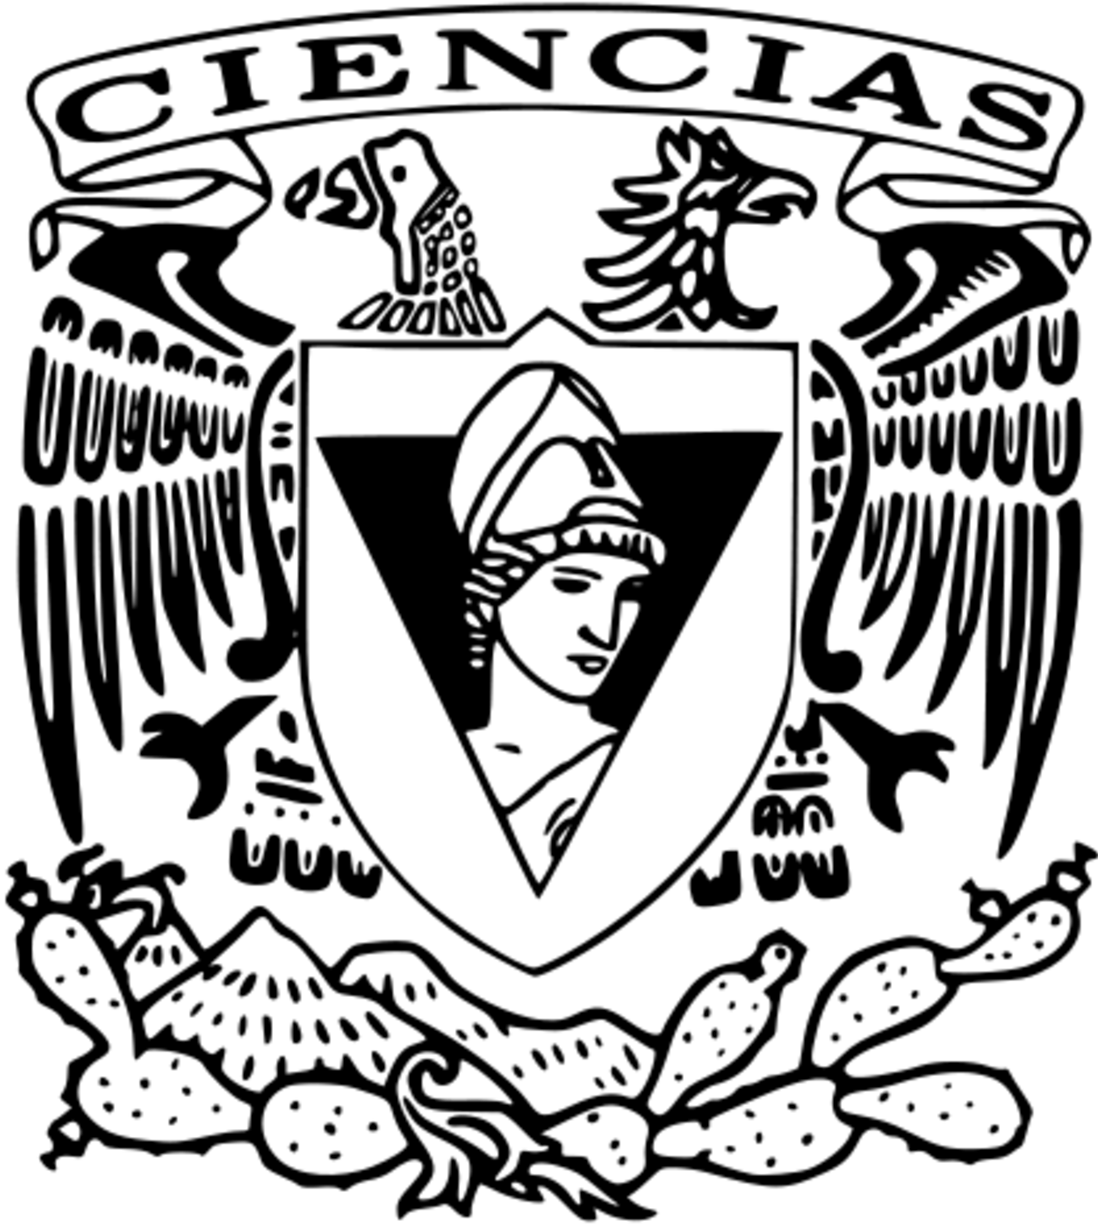
\includegraphics[height=3.3cm]{src/Img/Logo_FC.png}
    	\end{center}
    \end{minipage}
\end{center}


\rule{16.99cm}{0.1mm}

%------ Ejercicios -------- %
\begin{enumerate}
    \item \textbf{Descifrar el archivo file1.lol}
\begin{quote}
    Para el archivo \texttt{file1.lol} se comenzó inspeccionando su contenido binario en bruto,
    mostrando tanto los primeros caracteres en ASCII como en hexadecimal. El resultado
    no presentaba texto legible, sino bytes aparentemente aleatorios, lo que sugirió que se
    trataba de un cifrado clásico sobre bytes y no de una simple codificación.

    A continuación, se implementó un procedimiento en Python para probar de manera
    automática los cifrados César, Decimado y Afín, utilizando fuerza bruta sobre todas sus
    posibles claves. Una vez obtenido cada descifrado, se verificaba la cabecera con los
    \textit{magic bytes} característicos de distintos formatos (PDF, PNG, MP3, MP4).

    Para el caso del cifrado Afín, se utilizó la siguiente función que aplica la fórmula de
    descifrado con aritmética modular en $Z_{256}$:

    \vspace{.3cm}
    \begin{verbatim}
    def affine_decrypt(data, a, b):
        try:
            inv = pow(a, -1, 256)  # inverso modular de a
        except ValueError:
            return None
    
        result = bytearray()
        for byte in data:
            val = ((byte - b) * inv) % 256
            result.append(val)
        return result
    \end{verbatim}
    \vspace{.3cm}
    
    Tras las pruebas, se encontró que el método correcto era el \textbf{cifrado Afín} con
    parámetros $a=143$ y $b=157$. El archivo resultante comenzaba con la secuencia
    \texttt{0xFF 0xFB}, correspondiente al \textit{frame sync} de los archivos de audio MPEG
    Layer III (\texttt{.mp3}), lo que confirmó el formato.

    Una vez guardado el archivo descifrado, se verificó que podía reproducirse
    correctamente como audio. Con esto se validó el éxito del proceso de descifrado.
\end{quote}
\vspace{.5cm}

\end{enumerate}

\end{document}
